\ExamPart{Câu trắc nghiệm trả lời ngắn}{2}{}

\NQuestion Tìm số giá trị nguyên của $x$ thỏa mãn bất phương trình $x^2-4x-5<0$.

\NQuestion Trong mặt phẳng tọa độ $Oxy$, cho đường tròn $(C):x^2+y^2-2x+6y+6=0$. Tính bán kính của đường tròn.

\NQuestion Một khu vườn hình chữ nhật có chu vi $26$m và chiều dài hơn chiều rộng $3$m. Tính diện tích khu vườn.

\NQuestion Quỹ đạo của một vòi phun nước có dạng parabol như hình vẽ, với đỉnh ở độ cao $4$m và cắt mặt đất tại hai điểm cách gốc tọa độ $2$m về hai phía. Tính chiều cao của tia nước tại vị trí cách tâm $1$m.

\begin{center}
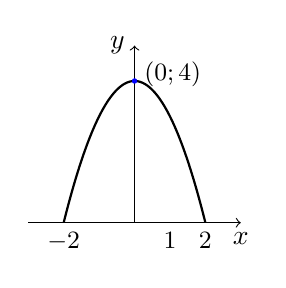
\begin{tikzpicture}[scale=0.45]
    \draw[->] (-3,0) -- (3,0) node[below] {$x$};
    \draw[->] (0,0) -- (0,5) node[left] {$y$};

    % y = 4 - x^2
    \draw[thick, domain=-2:2, samples=200] plot (\x,{4-\x*\x});

    \fill[color = blue] (0,4) circle (2.2pt);

    \node[right] at (0,4.2) {\small $(0;4)$};
    \node[below] at (-2,0) {\small $-2$};
    \node[below] at (2,0) {\small $2$};
    \node[below] at (1,0) {\small $1$};
\end{tikzpicture}

\end{center}
